\documentclass[11pt]{article}

% Language setting
% Replace `english' with e.g. `spanish' to change the document language
\usepackage[english]{babel}
\usepackage{float}
\usepackage{threeparttable}
\usepackage{tabularx}
\usepackage{nicefrac}
\usepackage{longtable} % for 'longtable' environment
\usepackage{pdflscape}
\usepackage[title]{appendix}

% Set page size and margins
% Replace `letterpaper' with`a4paper' for UK/EU standard size
\usepackage[letterpaper,top=2cm,bottom=2cm,left=3cm,right=3cm,marginparwidth=1.75cm]{geometry}

% Useful packages
\usepackage{amsmath,amssymb,amsthm}
\usepackage{graphicx}
\usepackage[colorlinks=true, allcolors=blue]{hyperref}

% https://tex.stackexchange.com/a/386936
\usepackage{thmtools}
\declaretheoremstyle[
spaceabove=6pt, spacebelow=6pt,
headfont=\normalfont\bfseries,
notefont=\mdseries, notebraces={(}{)},
bodyfont=\normalfont,
postheadspace=0.6em,
headpunct=:
]{mystyle}
\declaretheorem[style=mystyle, name=Hypothesis, preheadhook={\renewcommand{\thehyp}{H\textsubscript{\arabic{hyp}}}}]{hyp}
\usepackage{cleveref}
\crefname{hyp}{hypothesis}{hypotheses}
\Crefname{hyp}{Hypothesis}{Hypotheses}

% https://tex.stackexchange.com/a/113518
\newcommand\iid{i.i.d.}
\newcommand\pN{\mathcal{N}}

\title{Speculative Investment Behavior in Solar Energy Stocks}
\author{Stefan Yovchev}

\begin{document}
\maketitle

\newpage

\begin{abstract}
Following the signing of the Paris Climate Agreement in 2015, clean energy is now widely perceived not only as the way towards a carbon-neutral world, but also as a lucrative investment opportunity. This can be reflected in the price movements of clean energy stocks. Numerous indices, which track the green energy sector, have been outperforming the broad market by significant margins for the past two years and have delivered impressive returns at their peak in 2021. 
\newline

Green energy has enormous upside potential, which causes a lot of investors to flock into the market in an effort to gain exposure to the seemingly limitless growth of the clean energy industry. However, the question arises if this sudden investor interest might be the basis for a asset bubble in the sector. 
\newline

The following study investigates this question with regard to the solar energy market in particular, as solar energy might be a natural choice for investors due to the maturity and reliability of the technology. The paper studies price and returns data from January 2017 to January 2022 of the Invesco Solar ETF (TAN), which mirrors the MAC Global Solar Energy Stock Index (SUNIDX). First a 5-Factor Fama-French model is employed on weekly returns data in order to determine what the return dynamics and risks of solar energy stocks are. Additionally, a sup-augmented Dickey-Fuller (SADF) test and a generalized sup-augmented Dickey-Fuller (GSADF) test are applied on daily prices in order to identify explosive price behavior. 
\newline

The 5-Factor Fama-French model proves that solar energy companies carry significant idiosyncratic risk. The SADF and GSADF provide strong evidence to suggest the occurrence of multiple-bubble episodes during the sample period.

\end{abstract}

\newpage

\section{Introduction}

Amongst renewable energy sources, solar photovoltaics (PV) are considered to be a mature and reliable technology. In 2020 solar energy has generated over 800 TWh of power worldwide, which, in a sustainable development scenario, is projected to grow over six times until 2030 (IEA, 2021a). Solar photovoltaics are also on a steady upwards trajectory in their share in power and electricity generation. Table \ref{table:solar_share} shows the share of solar photovoltaics in the renewable electricity generation mix for 5 countries over the past 30 years. It is noticeable that solar energy is steadily becoming an ever important factor in the energy mix, even though hydroelectric and wind energy still account for the majority of the generated electricity from renewable sources. Nevertheless, in the same time-frame solar photovoltaics have seen exponential growth in terms of electricity generation worldwide -- in 1990 just 91 GWh have been generated by solar photovoltaics, whereas in 2019 that number has skyrocketed to over 680,000 GWh. This is an increase of over 74,000\%, compared to 3,670\% for wind energy and just 97\% for hydroelectric energy\footnote[1]{Based on IEA data from the IEA (2020), Renewables Information https://www.iea.org/data-and-statistics/data-product/renewables-information All rights reserved; as modified by Stefan Yovchev.}. Even though the latter two still have a greater share in the energy mix, there is little room to doubt solar's relevancy and it is hard to imagine that it's growth rate will stall or even decline in the future.

\begin{table}[!htbp] \centering 
    \label{table:solar_share}
    \caption[Caption for solar share]{
        Share of solar energy in renewable electricity generation by country \protect \footnote[1]}
    \begin{threeparttable}
        \begin{tabular}{@{\extracolsep{5pt}} lcccccccc} 
            \\[-1.8ex]\hline 
            \hline \\[-1.8ex] 
            Country or Region & 1990 & 1995 & 2000 & 2005 & 2010 & 2015 & 2020 \\ 
            \hline \\[-1.8ex] 
            Japan & 0.07\% & 0.11\% & 0.35\% & 1.53\% & 3.51\% & 25.92\% & 44.08\% \\ 
            India & 0.00\% & 0.00\% & 0.00\% & 0.00\% & 0.09\% & 5.73\% & 20.83\% \\ 
            EU 28 & 0.00\% & 0.01\% & 0.03\% & 0.34\% & 3.83\% & 12.99\% & 15.02\% \\ 
            USA & 0.00\% & 0.00\% & 0.06\% & 0.16\% & 0.76\% & 6.19\% & 14.66\% \\ 
            China & 0.00\% & 0.00\% & 0.01\% & 0.02\% & 0.09\% & 2.91\% & 12.98\% \\ 
            \hline \\[-1.8ex] 
        \end{tabular}  
    \end{threeparttable}
\end{table} 

With regard the technology's economical viability, the last decade has seen a steady decrease of the levelized cost of energy (LCOE) for photovoltaics, with a global weighted-average LCOE of around 0.057 \$/kWh in 2020, 85\% lower than in 2010 (IRENA, 2021). This marks the steepest decline in terms of costs amongst all renewable sources, as seen in Figure \ref{fig:lcoe}. Solar PV have significantly outperformed offshore wind, yet onshore wind and hydro energy still provide a lower LCOE, which, however, may change in the next few years. According to IRENA's Renewable Auction and PPA Databas, utility-scale solar projects, planned for 2022, are projected to average a price of 0.04 \$/kWh, which is slightly less than onshore wind's projected average price of 0.043 \$/kWh (IRENA, 2021). Additionally, in the last 10 years hydro energy has almost consistently seen slight year-over-year increases of it's LCOE. This may pave the way for solar PV to become the most cost-efficient technology in the future.
\newline


\begin{figure}[h]
    \centering
    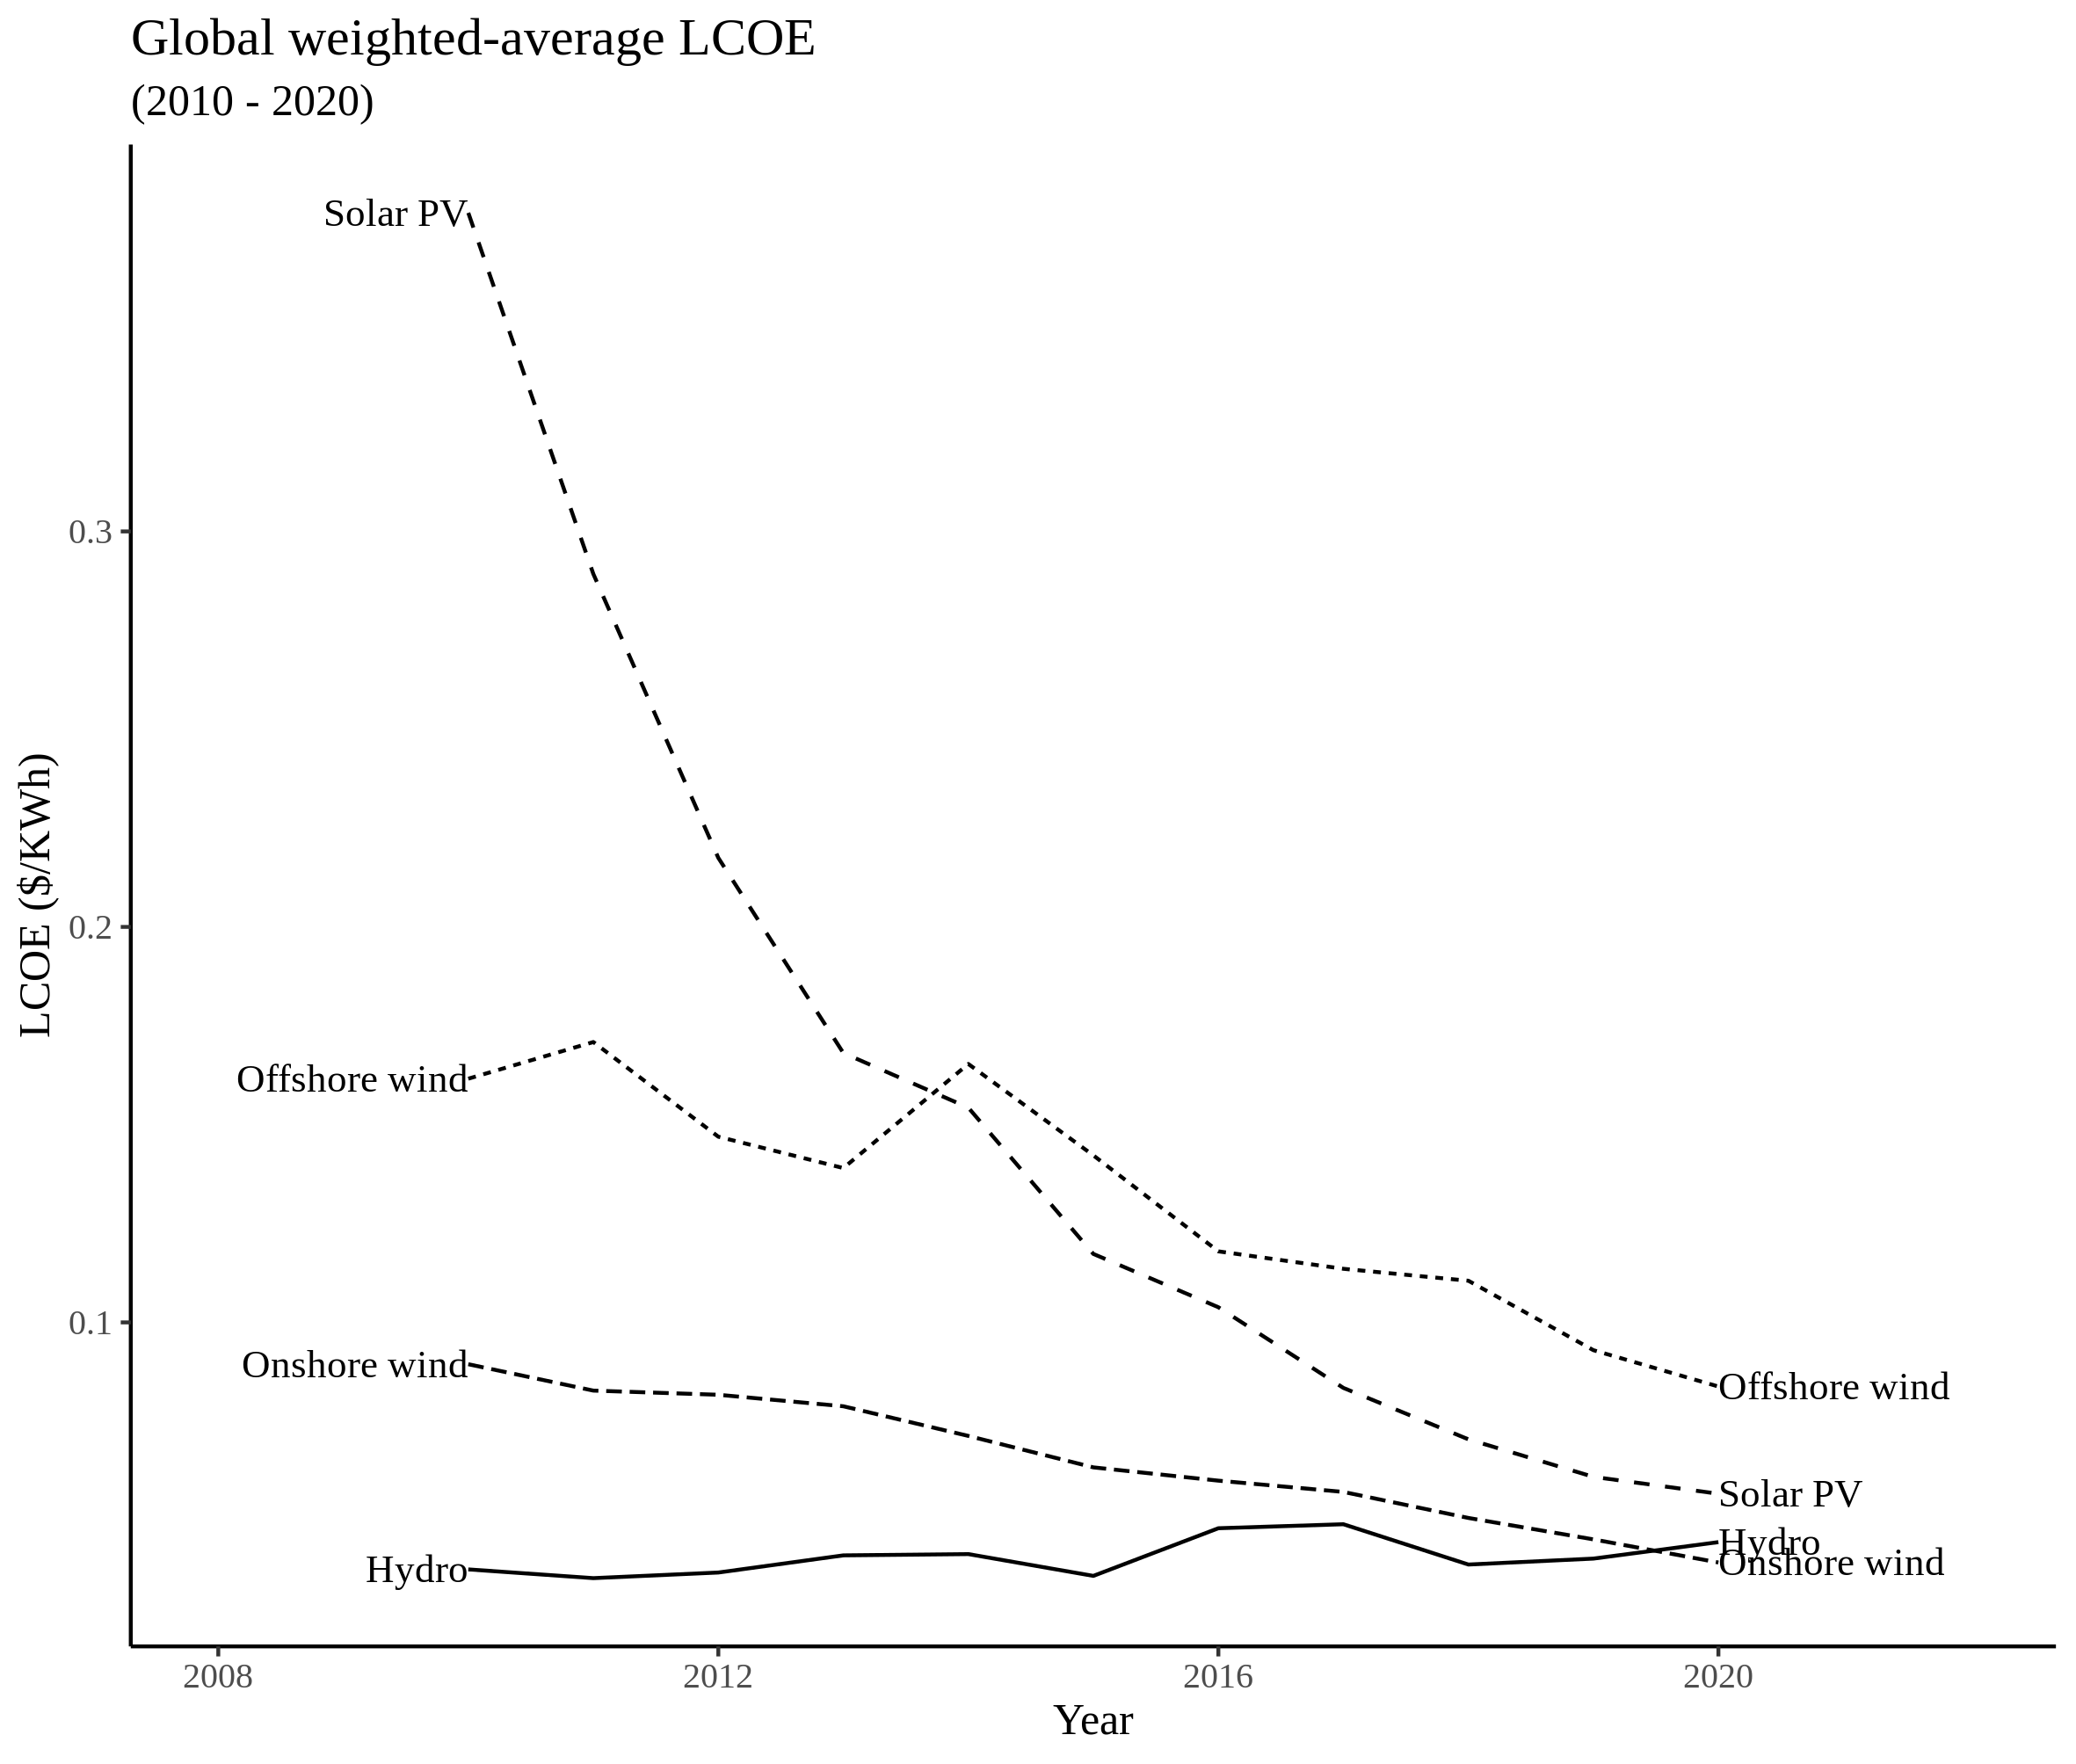
\includegraphics[width=\textwidth]{Figures/LCOE.png}
    \caption{LCOE of selected renewable technologies}
    \label{fig:lcoe}
\end{figure}

The developments over the past decade, plus the strong government support, which green energy as a whole receives, make out companies in the solar energy sector an alluring financial investment to both investment funds and retail investors. According to data provided by Bloomberg New Energy Finance, over \$3.6 billion has been put into solar energy companies on the primary stock market in 2019, accounting for more than half of the investments in clean energy (FS-UNEP, 2020). This amount, however, was less than half of the investments made in 2015, which marks the peak for solar energy stocks on the primary market. This reinforces the notion of solar's mature and well-established nature -- publicly traded companies do not need to issue new stock in order to finance their projects, as they can do so from their own cash-flows. Additionally, there are less IPOs of new companies, which in turn provides less opportunities for investors to tap into up and coming companies.
\newline

The secondary market for solar energy stocks, however, paints a vastly different landscape. There appears to be a lot of positive investor sentiment towards this sector, which can be seen in the movements over the last few years of the MAC Global Solar Energy Stock Index (SUNIDX), mirrored by the Invesco Solar ETF (TAN). Since 2017 solar energy stocks have outperformed the broader market to date. Additionally, they have outperformed the market on a per-year basis in three of the last five years -- 2017, 2018, and 2020. Figure \ref{fig:clean_energy_stocks_vs_broader_market} compares the daily returns of the Invesco Solar Energy ETF to the returns of ETFs which seek to mirror broader market indices -- S\&P 500 (SPY) and MSCI World (URTH).
\newline

\begin{figure}[h]
    \centering
    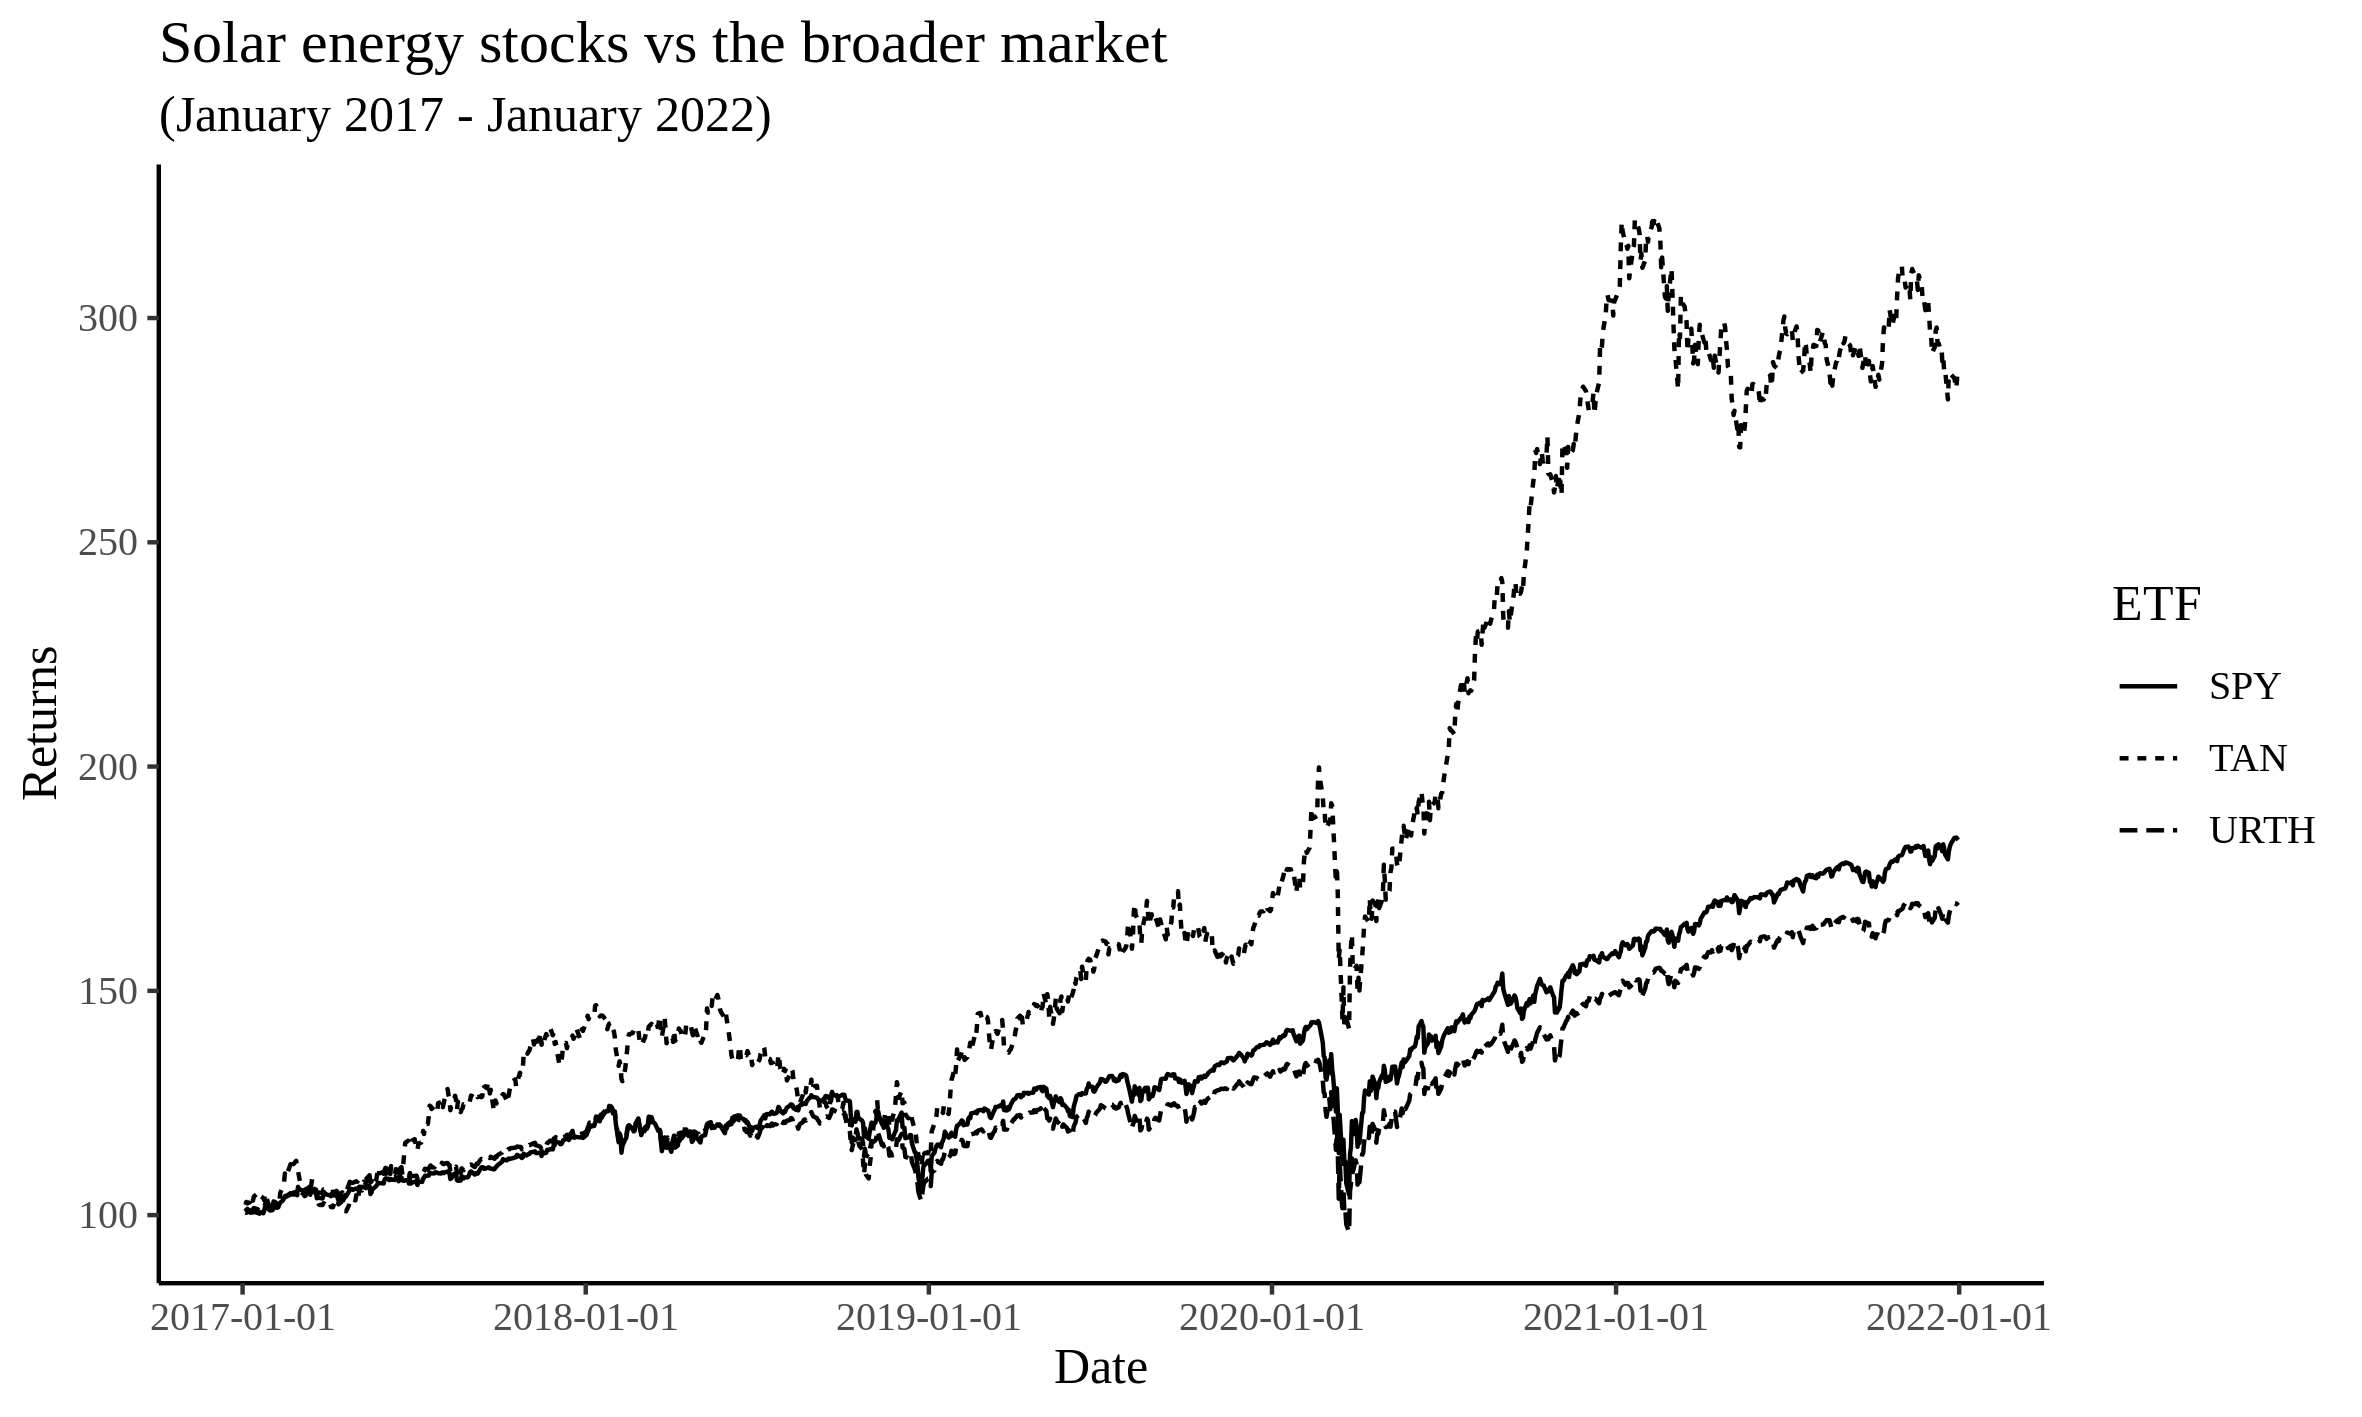
\includegraphics[width = \textwidth]{Figures/Solar energy stocks vs the broader market.png}
    \caption{Daily returns of selected ETFs}
    \label{fig:clean_energy_stocks_vs_broader_market}
\end{figure}

As depicted above, since the time shortly after the Paris Climate Agreement (November 2016) has come into effect solar stocks are in a impressive bull run, with periods of significant out-performance of the market, especially in the aftermath of the March 2020 crash, when solar energy stocks have shot up in price several times more than the overall market. Even thought 2021 has been a volatile year for these stocks their to-date returns have remained notably higher and would require a massive crash to drop below the levels of the broader market.
\newline

Solar energy's relevancy and its prospects of immense growth in the next decades have already established  and as such, many investors seek exposure to solar's seemingly endless potential which, naturally, comes with the expectation of great returns in the future. However, the question arises as to how much the price movements of the last few years reflect the true present valuation of the companies and not so much the investors' hope of what these valuations might be in the next 5, 10 or 20 years. This is reminiscent of the dot-com bubble of the late 1990's and early 2000's, as the Internet had been perceived as the future and with tech and Internet companies of the time seemingly promising substantial returns with nothing in their way to stop them. Naturally, the investors back then had wanted a share of this newfound rage, thus pricing those companies for a hypothetical future, not truly reflecting what they were worth in that moment. And thus one might ask themselves: are we witnessing the same now with clean energy?

\newpage

\section{Literature Review}

The dynamics of clean energy stock returns is a topic that has been slowly garnering the interest of researchers over the past several years, but even still the existing literature is relatively scarce. The main question, which researchers have sought to answer regards the factors that influence the price movements of these stocks.
\newline

Several studies have analyzed this question in the context of equity markets. That is to say -- which asset's price movements appear to impact the movements of clean energy stocks' prices? It has been empirically proven in numerous studies that there is three market factors which may significantly influence stocks of renewable energy companies: oil, technological stocks, and interest rates. On a conceptual basis, such a relationship makes sense. Firstly, oil is a symbol of the traditional, "dirty" energy sector, so a significant relationship between it and clean energy is to be expected. Secondly, clean energy, like any industry, is dependent on the advancements in technology, but even more-so than other sectors. Finally, interest rates are always a non-negligible factor in explaining stock return dynamics. The fundamental model of asset pricing, the capital asset pricing model (CAPM), explains excess returns of a security via the risk-free rate of return and the market risk premium (Sharpe, 1964; Lintner 1965).
\newline

Henriques and Sadorsky (2008) first hypothesize that there is a significant relationship between prices of renewable energy stocks and the three aforementioned assets. They develop and estimate a four-variable vector autoregressive model (VAR), which yields back statistically significant results, proving this relationship. Additionally, the study proves that tech stocks and oil prices Granger cause the prices of clean energy stocks. Later on, Kumar et al. (2012) further extend this model by including carbon prices as an explanatory variable. Carbon pricing is widely viewed as a necessary mechanism in fighting climate change, thus the logical assumption can be made that a carbon price might be a significant driver for investments in clean energy companies. A five-factor VAR-model is used in the study, but it is not able to prove a statistically significant relationship between carbon prices and clean energy stock prices. Nevertheless, the results reaffirm previous results about the return dynamics of clean energy stocks.
\newline

With the use of multivariate GARCH models, Sadorsky (2012a) examines the correlations and volatility dynamics between the prices of oil, renewable energy stocks, and technological stocks. Amongst the employed models, the dynamic conditional correlation MGARCH model serves to best explain the co-movements of the different assets and provides evidence that prices of renewable energy companies have a stronger correlation with the prices of technological stocks, as opposed to those of oil. The interplay between these securities has further been proven in the following years by several other studies each of which applies a different econometric model or technique -- Markov switching VAR (Managi and Okimoto, 2013), multi-factor asset pricing model with timevarying coefficients (Inchauspe et al., 2015), cointegration and Granger causality tests (Bondia et al., 2016).
\newline

The return dynamics of clean energy stocks can also be studied in the context of common risk factor models, such as the 3-Factor Fama-French (1992), 4-Factor Carhart (1997), or 5-Factor Fama-French (2015) models. These models seek to capture stock return dynamics by building up on the CAPM, by factoring in not only systematic (market) risk, but also company-specific characteristics. Sadorsky (2012b) finds that companies in the clean energy sector have higher systematic risk, which can be offset by a company's sales growth, but at the same time can also be increased by a rise in oil prices. Bohl et al. (2015) also estimate high betas for the market risk premium factor, which implies that renewable energy stocks have above-average risk. Their study also finds that the monthly risk-adjusted returns are negative. These findings are also echoed by Sokolovska \& Kešeljević (2019), which estimate market betas above 1, as well as negative alphas. With regard to the company characteristics, they conclude that stocks in the sector tend to be small-cap, contrarian growth stocks.
\newline

Some researchers try to find factors influencing the prices for alternative energy stocks outside of the market itself. Geopolitical events, political decisions or natural disasters can all have varying degrees of impact on investor sentiment towards clean energy. Zhao (2020) finds that policy uncertainty has a negative impact on price movements, whilst, on the other hand, shocks in the oil market resulting from a supply decrease have a positive effect. Schütze et al. (2020) find that international climate negotiations send a positive signal to investors in "green" companies. Antoniuk \& Leirvik (2021) employ an extensive event study to investigate the reaction of the clean energy stock market to various global events, such as the Fukushima disaster in 2011 or the signing of the Paris Climate Agreement in 2015, both of which proved to have a positive impact.
\newline

All this ties into the question as to how much of the price movements in alternative energy stocks are driven by the described market forces and how much is driven by speculative behavior. Bohl et al. (2013) study explosive price behaviors in the German clean energy stock market and conclude that there was a speculative bubble in the market during the mid-2000s. Similar results were found by Bohl et al. (2015) for the European markets for clean energy stocks. Both studies make use of a sup augmented Dickey-Fuller test (Phillips et al., 2011, 2012).
\newline

Most of the literature which deals with the topic of clean energy stocks considers the sector as a whole, with analysis of separate sub-sectors of alternative energy, like wind or solar stocks, for example, are few and far between. This is why this study will consider the solar sector only, not only because of it's rapid growth which is projected to go into the future, as outlined in the introductory section, but because of the space in which solar energy operates as a business. Solar PV projects can range vastly in terms of scale -- from large utility-scale projects to small residential rooftop installations. This consumer facing side of solar energy can be seen as a leverage point for solar PV as opposed to other energy sources, in that there is a potentially larger market to sell to. According to IEA (2020) between 2023 and 2025 the residential segment of Solar PV is set to grow between 6\% and 40\%, whilst utility-scale capacities are projected to grow between 2\% and 27\%.

\newpage
\section{Data \& Methodology}
\subsection{Invesco Solar ETF}
In the same vein as the mentioned literature, this study will focus on a stock index, which seeks to capture the solar energy sector -- MAC Global Solar Energy Index (SUNDIX). The index includes 42 stocks of companies which are part of the whole supply chain -- raw materials, manufacturing, installment, operating (in both solar PV and solar thermal technologies), as well as companies which manufacture and develop solar-related equipment. The SUNDIX uses modified market cap weighting to construct its portfolio, in order to guarantee maximum exposure to the solar energy sector. For this it uses so-called Solar Exposure Scores (SES), which are defined as follows: 
\begin{itemize}
    \item if more than \nicefrac{2}{3} of a company's revenue is derived from solar-related activities they get assigned a SES of 1.0,
    \item if between \nicefrac{1}{3} and \nicefrac{2}{3} of a company's revenue is derived from solar-related activities they get assigned a SES of 0.5,
    \item if under \nicefrac{1}{3} of a company's revenue is derived from solar-related activities, the company is not included in the index.
\end{itemize}
The Solar Exposure Scores are then further used to determine the percentage of a company's market cap to be used in the weighting process. For companies with a SES of 0.5 only 50\% of their market cap will be considered in the weighting, thus reducing their raw weight by half. Appendix A provides detailed information on the stocks included in the index.
\newline

In order to gather price information about the index the study will sample daily data for the Invesco Solar ETF (TAN) which mirrors the SUNDIX. Following the conclusions of Antoniuk \& Leirvik (2021) with regard to the stock market response to the signing of the Paris Climate Agreement, the sample period is decided to be 01.01.2017 - 01.01.2022. The assumption is made that the event of the Paris Agreement coming into force (04.11.2016), and not the signing of the agreement in 2015, marks the beginning of a new investment climate for clean energy stocks. Additionally, the sample period is offset by two months from the implementation of the Paris Agreement in order to control for any potential bias, introduced from reactionary market responses and eventual sell-offs.
\newline

The data is accessed via the Yahoo Finance API and contains observations for 1,259 trading days. The price for a given trading day is determined by the price of the ETF at market close. Table \ref{TAN_daily_prices_summary} provides summary statistics for the price data.

% Table created by stargazer v.5.2.2 by Marek Hlavac, Harvard University. E-mail: hlavac at fas.harvard.edu
% Date and time: Wed, Mar 30, 2022 - 03:13:31 PM
\begin{table}[!htbp] \centering 
  \caption{Summary statistics TAN daily prices (January 2017 - January 2022)} 
  \label{TAN_daily_prices_summary} 
\begin{tabular}{@{\extracolsep{5pt}}lcccccc} 
\\[-1.8ex]\hline 
\hline \\[-1.8ex] 
Statistic & \multicolumn{1}{c}{N} & \multicolumn{1}{c}{Mean} & \multicolumn{1}{c}{St. Dev.} & \multicolumn{1}{c}{Min} & \multicolumn{1}{c}{Median} & \multicolumn{1}{c}{Max} \\ 
\hline \\[-1.8ex] 
TAN & 1,259 & 41.706 & 28.155 & 16.960 & 27.010 & 121.940 \\ 
\hline \\[-1.8ex] 
\end{tabular} 
\end{table} 

\begin{figure}
    \centering
    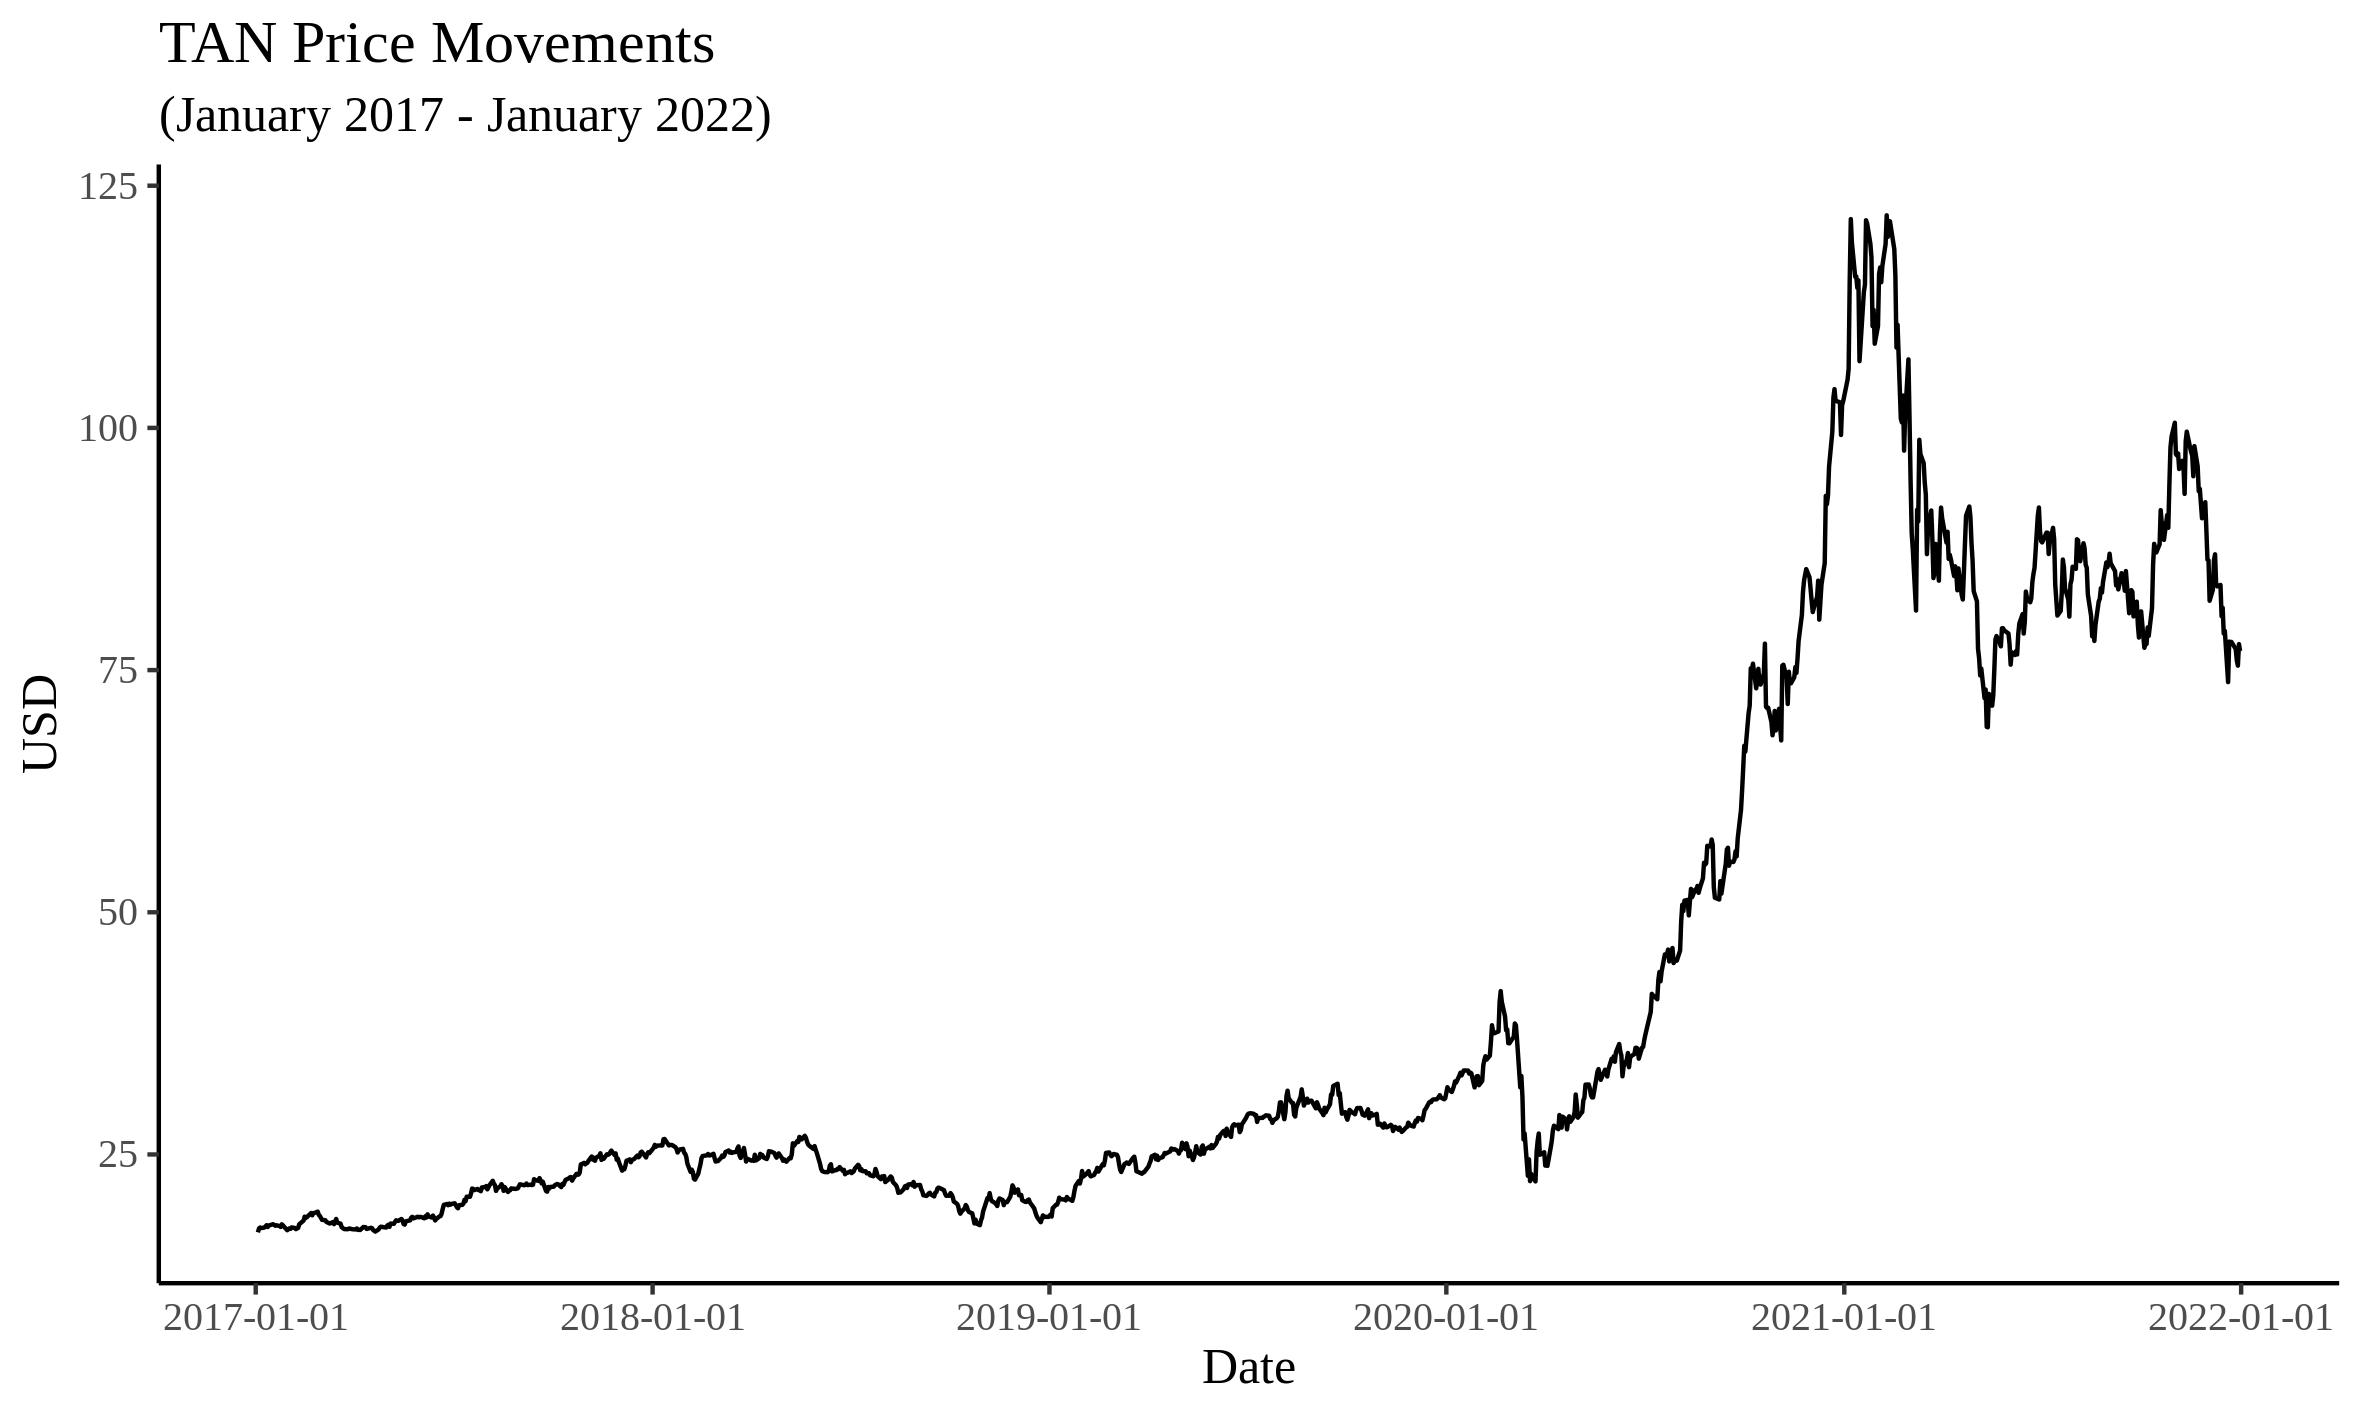
\includegraphics[width=\textwidth]{Figures/TAN prices.png}
    \caption{TAN Daily prices}
    \label{fig:TAN_daily_prices}
\end{figure}

As can be seen in Figure \ref{fig:TAN_daily_prices} solar stocks have been on a slow upwards trajectory in the first three years of our sample period. However, in March of 2020 as the financial world went into a bear market, following the beginning of the global COVID-19 pandemic, the prices of the TAN reached their mid-2018 levels, wiping out almost two years worth of gains. Following this event the markets started to slowly recover with the introduction of financial policies easing the impact of the pandemic. Solar energy stocks started a new upward trajectory at rates much higher than those of the broader market. This explosive price behavior continued until the beginning of 2021 when it reached its peak before an eventual sell-off, with prices still much above the average price of the ETF for the sample period of 41 USD. This period (June 2020 - January 2021) could potentially be a bubble episode.

\subsection{Multi-Factor Model}

Understanding the relationship between risk and returns is of great importance to investors. The original model which addresses this problem is the single-factor CAPM introduced in 1964 by William Sharpe. In the following decades different models have been developed which add new factors which might explain a security's returns. The most famous multi-factor model was developed by Fama and French in 1993 by extending the CAPM with two additional factors -- the size of firms and the book-to-market ratio. These two factors, called small-minus-big (SMB) and high-minus-low (HML), respectively, track the out-performance of small-cap stocks vs large-cap stocks and the out-performance of value stocks vs growth stocks. In 2015 Fama and French add two more factors -- profitability and investment. The profitability factor, robust-minus-weak (RMW) captures the difference in the returns of companies with robust operating profitability to those with a weak one. Similarly, the investment factor, conservative-minus-aggresive (CMA), compares companies with either a conservative or aggressive internal investment policy. 
\newline

The 5-Factor Fama-French model can thus allow for a better understanding of the return dynamics of the TAN ETF, as well as the risk factors which play a role in its returns. 
\newpage

The model can be defined as follows:

\begin{equation}
\label{eq:ff_regression}
R_{TAN,t} - R_{f,t} = \alpha_t + \beta_1(R_{Mkt,t}-R_{f,t}) + \beta_2SMB_t + \beta_3HML_t + \beta_4RMW_t + \beta_5CMA_t + \epsilon_t
\end{equation}

With $R_{TAN,t}$ defined as the returns of the TAN, $R_{f,t}$ -- the risk-free rate of return. The difference of both, $R_{TAN,t} - R_f$, gives the expected excess returns. $R_{Mkt,t}$ are the market returns and $R_{Mkt,t} - R_{f,}$ -- the market risk premium. $\beta_{1,...,5}$ are the factor coefficients, $\epsilon_t$ is the regression error term (\iid~$\epsilon  \sim \pN(0, \sigma^2)$), and $\alpha_t$ measures the excess returns.
\newline

Data for the five factors is kindly provided by Kenneth Fama on his personal website (\url{https://mba.tuck.dartmouth.edu/pages/faculty/ken.french/Data_Library/f-f\_5\_factors_2x3.html}) in the form of benchmark portfolios with daily returns for each factor accessible from July 1964 until now. This study will estimate the 5-Factor Fama-French model on weekly returns of the TAN. Table \ref{ff_summary} provides summary statistics.

% Table created by stargazer v.5.2.2 by Marek Hlavac, Harvard University. E-mail: hlavac at fas.harvard.edu
\begin{table}[!htbp] \centering 
  \caption{Summary statistics on weekly returns of TAN and the 5 Fama-French factors for the sample period} 
  \label{ff_summary} 
\begin{tabular}{@{\extracolsep{5pt}}lrrrrrr} 
\\[-1.8ex]\hline 
\hline \\[-1.8ex] 
Statistic & \multicolumn{1}{c}{N} & \multicolumn{1}{c}{Mean} & \multicolumn{1}{c}{St. Dev.} & \multicolumn{1}{c}{Min} & \multicolumn{1}{c}{Median} & \multicolumn{1}{c}{Max} \\ 
\hline \\[-1.8ex] 
$R_{TAN}$ & 261 & 0.707 & 5.384 & $-26.360 & 0.634 & 17.420 \\ 
$R_{Mkt} - R_f$ & 261 & 0.334 & 2.560 & $-14.561 & 0.490 & 12.336 \\ 
SMB & 261 & $-0.034 & 1.551 & $-7.671 & $-0.172 & 4.764 \\ 
HML & 261 & $-0.162 & 2.164 & $-8.153 & $-0.232 & 9.640 \\ 
RMW & 261 & 0.096 & 1.128 & $-3.635 & 0.034 & 4.114 \\ 
CMA & 261 & $-0.044 & 0.887 & $-2.947 & $-0.111 & 3.096 \\ 
\hline \\[-1.8ex] 
\end{tabular} 
\end{table}

\subsection{Univariate Right-Tailed Tests}
The focal point of this study is testing for explosive price behavior. This is done by employing two methodologies -- the sup-augmented Dickey-Fuller (SADF) test (Phillips et al., 2011) and the generalized SADF (GSADF) test (Phillips et al., 2015). Both build upon the original augmented Dickey-Fuller (ADF) test (Dickey \& Fuller, 1979), which tests the null hypothesis that there is a presence of a unit-root in a time-series. As per Pavlidis et al. (2017), the standard ADF can be defined as follows:

\begin{equation}
\label{eq:adf_regression}
\Delta y_t = \alpha_{r_1, r_2} + \beta_{r_1, r_2} y_{t-1} + \sum_{j=1}^k \psi_{r_1, r_2}^{j} \Delta y_{t-j} + \epsilon_t 
\end{equation}

With $\Delta y_t$ being generic a time series and $\Delta y_{t-j}, j = 1, ..., k $ its lagged first differences. $\alpha_{r_1, r_2}, \beta_{r_1, r_2}, \psi_{r_1, r_2}^j, j = 1, ..., k$ are the regression coefficients, $\epsilon_t$ is the error term of the regression (\iid~$\epsilon  \sim \pN(0, \sigma^2)$). $r_1$ and $r_2$ mark sample beginning and sample end, respectively.

Setting $r_1$ = 0 and $r_2$ = 1 gives the full sample period and as such the $ADF_0^1$ test statistic equals $\frac{\hat{\beta}_{0,1}}{SE(\hat{\beta}_{0,1})}$, for which the null and alternative hypothesis are

\setcounter{hyp}{-1}
\begin{hyp} \label{hyp:a} $\beta_{0,1} = 0$ \end{hyp}
\begin{hyp} \label{hyp:b} $\beta_{0,1} > 0$ \end{hyp}
\newline

Under the null-hypothesis the $ADF_0^1$ has the following limit distribution:

$$ \frac{\int_0^1 WdW}{(\int_0^1 W^2)^\frac{1}{2}} $$

with $W$ being a Wiener process (Brownian motion). Testing for explosive behavior requires comparing the $ADF_0^1$ statistic to the right-tailed critical value of the limit distribution, whereby if this value is exceeded the null hypothesis is rejected.
\newline

The limitation of the standard ADF is that it can test for exuberance for the entirety of the sample data. Phillips et al. (2011) tackle this issue by introducing a recursive procedure for estimating (\ref{eq:adf_regression}) based on subsamples of the data -- the SADF. This model relies on an window, $r_2$, which has a fixed beginning at $r_1 = 0$ and is forward increasing, $r_2$ \in [$r_1$, 1], with 1 marking the end of the sample. The result of this recursive estimation is a series of $ADF_0^{r_2}$ test statistics, the supremum of which, the SADF statistic, being 

$$ SADF(r_0) = \sup_{r_2 \in [r_0, 1]} ADF_0^{r_2} $$

with a limit distribution under the null

$$ \sup_{r_2 \in [r_0, 1]} \frac{\int_0^{r_2} WdW}{(\int_0^{r_2} W^2)^\frac{1}{2}} $$

\newline
The null and alternative hypotheses for the SADF test are the same, however the SADF allows for the detection of explosive movements within the sample period and not for the whole period itself, should the null be rejected.
\newline

Finally, the GSADF (Phillips et al., 2015) allows for the detection of multiple regime switches within the sample period. This is achieved by relaxing the requirement of a fixed window start, $r_1$, thus allowing for more flexibility. The GSADF statistic is given by:

$$ GSADF(r_0) = \sup_{r_2 \in [r_0, 1], r_1 \in [0, r_2 - r_0]} ADF_{r_1}^{r_2} $$

Its respective limit distribution is defined as

$$  \sup_{r_2 \in [r_0, 1], r_1 \in [0, r_2 - r_0]} \frac{\frac{1}{2} r_w [W(r_2)^2 - W(r_1)^2 - r_w] - \int_0^1 W(r)dr[W(r_2) - W(r_1)]}{r_w^{\frac{1}{2}}(r_w\int_{r_1}^{r_2} W(r)^2dr - [\int_{r_1}^{r_2}W(r)dr]^2)^\frac{1}{2}} $$

Again, a rejection of the null hypothesis entails the presence of multiple bubble-like sub-periods within the sample period.
\newline

This study applies both the SADF and GSADF methodologies to the daily price data of TAN in order to detect the presence of explosive price behavior in the stock market for solar energy companies. As outlined in Section 3.1. a potential bubble episode might have occurred in the second half of 2020 with a bust some time in 2021. Following Phillips et al. (2015), $r_0$, the initial window length, is set to 0.10 (the initial sub-sample period thus becomes 125 trading days). Additionally, a lag of 1 traing day is used for both regressions. The critical values for each test statistic, at the 99\%, 95\%, and 90\% significance level, are calculated with the use of Monte Carlo simulations with a 1,000 replications.    

\newpage

\section{Results}

\subsection{Return dynamics of solar energy stocks}

Ordinary least-squares (OLS) are applied in order to estimate (\ref{eq:ff_regression}). Table \ref{ff_5_factors_results} provides the regression results.

\begin{table}[!htbp] \centering 
    \caption{Regression results of Fama-French 5-Factor Model} 
    \label{ff_5_factors_results} 
    \begin{threeparttable}
        \begin{tabular*}{\textwidth}{@{\extracolsep{\fill}}rrllrl} 
            \\[-1.8ex] 
            \hline
            \hline
            \\[-1.8ex] 
            Variable & Estimate & & Std. Error & t value & Pr($> |$t$|$) \\ 
            \\[-1.8ex] 
            \hline
            \\[-1.8ex] 
            $\alpha$ & $0.312$ & & $0.231$ & $1.352$ & $0.172$ \\ 
            $R_{Mkt} - R_f$ & $1.217$  & *** & $0.095$ & $12.783$ & $0.000$ \\ 
            SMB    & $0.816$  & *** & $0.184$ & $4.444$  & $0.000$ \\ 
            HML    & $-0.320$ & *   & $0.158$ & $-2.032$ & $0.044$ \\ 
            RMW    & $-0.740$ & **  & $0.247$ & $-2.993$ & $0.003$ \\ 
            CMA    & $-0.735$ & *   & $0.308$ & $-2.390$ & $0.018$ \\ 
            \\[-1.8ex] 
            \hline
            \\[-1.8ex] 
        \end{tabular*} 
        \begin{tablenotes} 
            \footnotesize
            \item Adjusted R$^{2}$:  0.5445; F-statistic: 63.16$^{***}$
            \item \textit{Note:} $^{*}$p$<$0.1; $^{**}$p$<$0.05; $^{***}$p$<$0.01
        \end{tablenotes} 
    \end{threeparttable}
\end{table} 

The adjusted $R^2$ of 0.5445 indicates that around half of the total risk is idiosyncratic, meaning that almost 50\% of the risk in the TAN ETF stems from the firms themselves. This is not risk carried over by the overall market dynamics, but rather uncertainty on a micro-economic level, specific to each individual stock. Idiosyncratic risk can not be diversified away, which is something which investors in the solar energy market should take into consideration.
\newline

A statistically significant $\beta_1$ of 1.217 for the market risk premium entails that solar energy stocks do have abnormal risk compared to the overall market, although not too high. The regression results for the SMB ($\beta_2$) and HML ($\beta_3$) factors indicate findings similar to those of Sokolovska \& Kešeljević (2019), in that solar energy stocks tend to be small-cap growth stocks. The growth stock characteristic of the solar energy companies is similar to that of tech companies, which might explain why some investors perceive both assets to be comparable. Another common characteristic between technology and solar energy stocks is that of the frims' investment strategies, captured by the CMA factor. The negative $\beta_5$ is indicative that solar energy companies have a preference for more aggressive investment policies. Finally, the estimation for the RMW factor ($\beta_4$) suggests that companies in the TAN ETF have weak operating profitability. 
\newline

The results of the 5-Factor model estimation are conclusive that solar energy stocks have carried significant risk in the sample period. High risk might be deemed attractive for some investors, since it is associated with high returns. The risk-adjusted returns ($\alpha$) of the regression is positive at $0.312$\% (16.2\% p.a.) which, although not statistically significant, suggests that solar energy stocks have been good performers. Still, the question remains as to how much of this out-performance can be attributed solely on the good financial performance of the companies themselves over the sample period and how much is driven by investor speculation.

\subsection{Bubble episodes in solar energy stocks}
In the following section the results of the SADF and GSADF tests will be discussed. The results of the SADF and GSADF, along with the critical values of each test statistic can be found in Table \ref{df_test_results}.

% Table created by stargazer v.5.2.2 by Marek Hlavac, Harvard University. E-mail: hlavac at fas.harvard.edu
% Date and time: Fri, Apr 01, 2022 - 07:31:15 AM
\begin{table}[!htbp] \centering 
  \caption{Results of univariate right-tail tests} 
  \label{df_test_results} 
\begin{tabular}{@{\extracolsep{5pt}} llrrrr} 
\\[-1.8ex]\hline 
\hline \\[-1.8ex] 
Test & t-stat & 90\% & 95\% & 99\% \\ 
\hline \\[-1.8ex] 
SADF & $7.217^{***}$ & $1.274$ & $1.545$ & $2.046$ \\ 
GSADF & $7.217^{***}$ & $1.947$ & $2.216$ & $2.720$ \\ 
\hline \\[-1.8ex] 
\end{tabular} 
\end{table} 

Both the SADF and GSADF tests reject $H_0$ at the 1\% significance level, meaning that explosive price behavior can be observed within the sample period. Figures \ref{fig:SADF_results} and \ref{fig:GSADF_results} illustrate when these episodes have occurred. The shaded areas represent a bubble episode, which occurs when the t-stat exceeds the right-tail critical value of either the SADF or GSADF limit distribution. As can be seen, the assumption that a bubble was present in the period from mid-2020 to early 2021 holds true. 

\begin{figure}[!h]
    \centering
    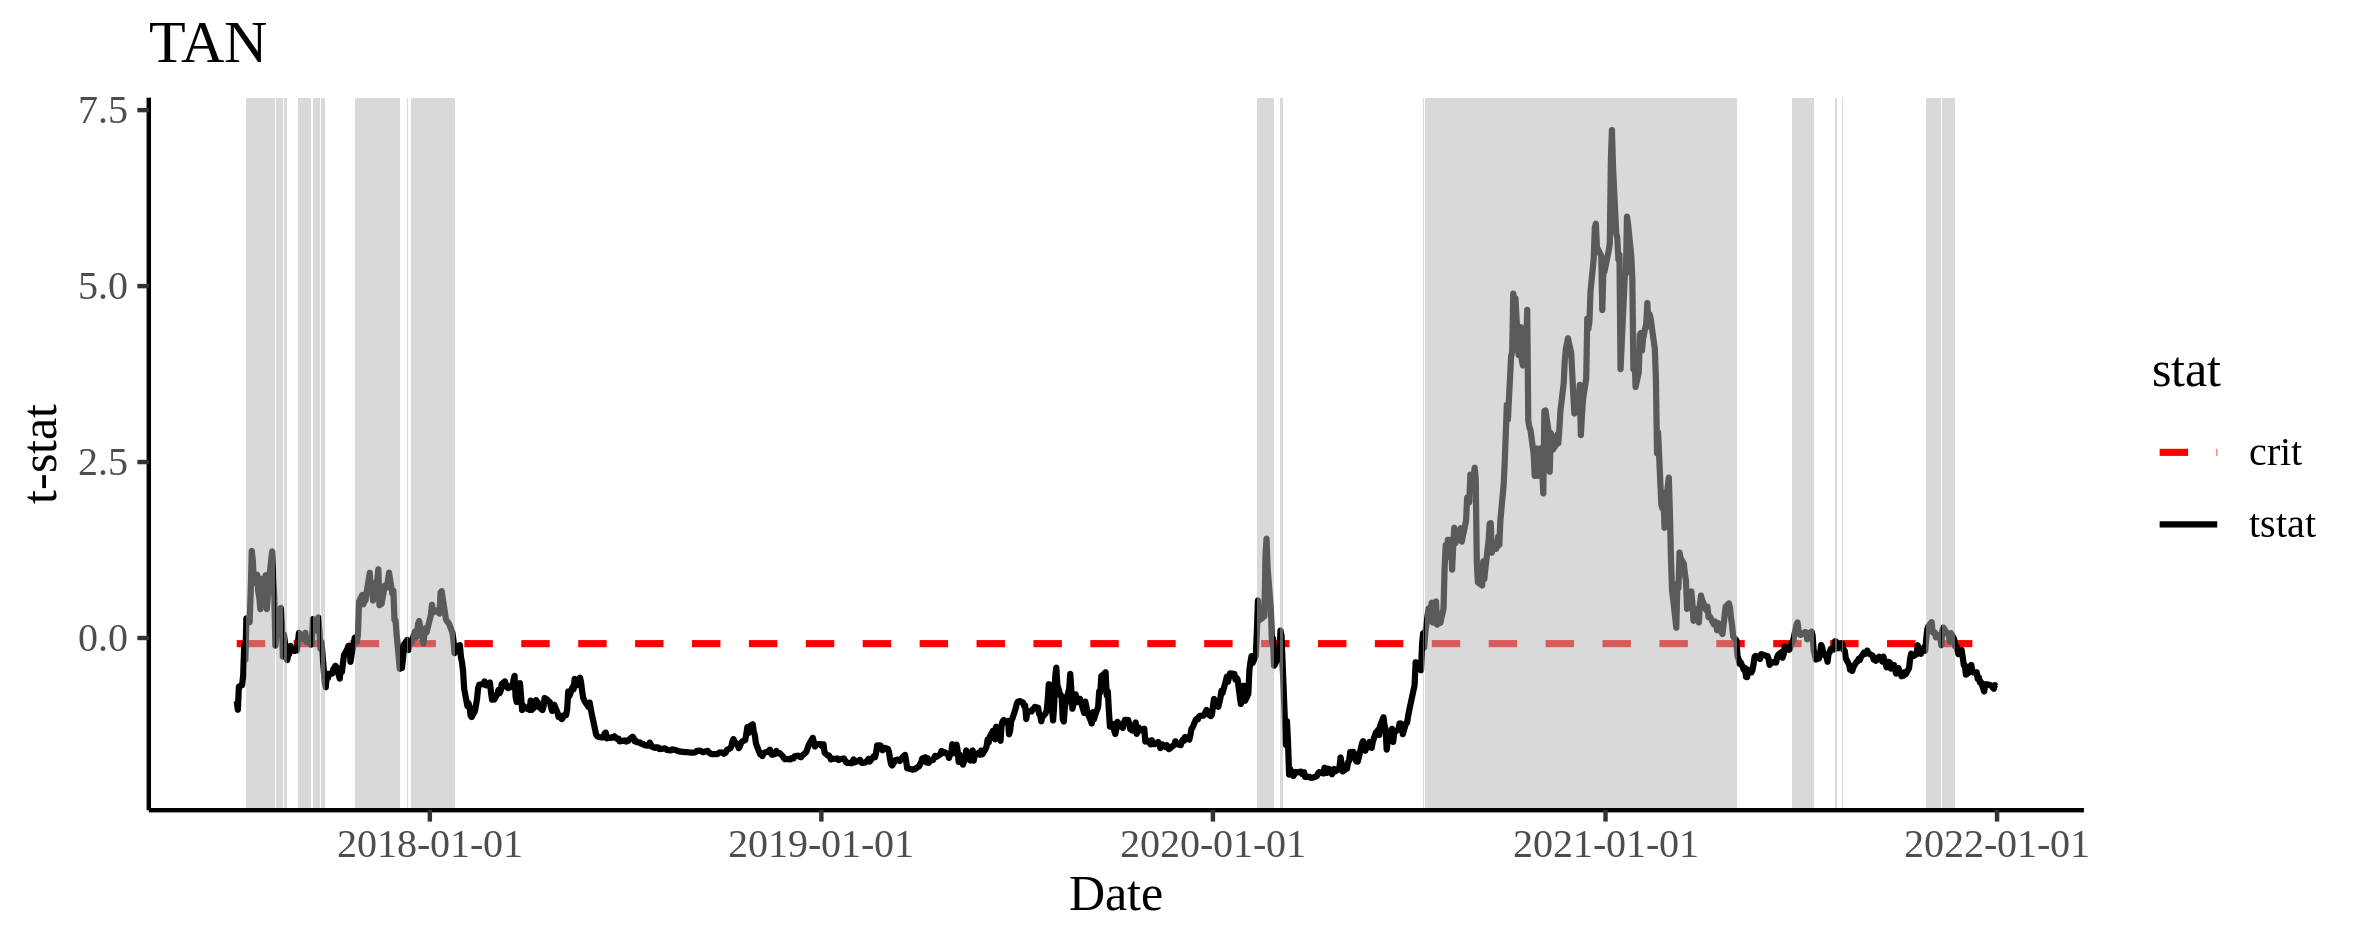
\includegraphics[width=\textwidth]{Figures/sadf_prediciton.png}
    \caption{SADF Results}
    \label{fig:SADF_results}
\end{figure}

\begin{figure}[!h]
    \centering
    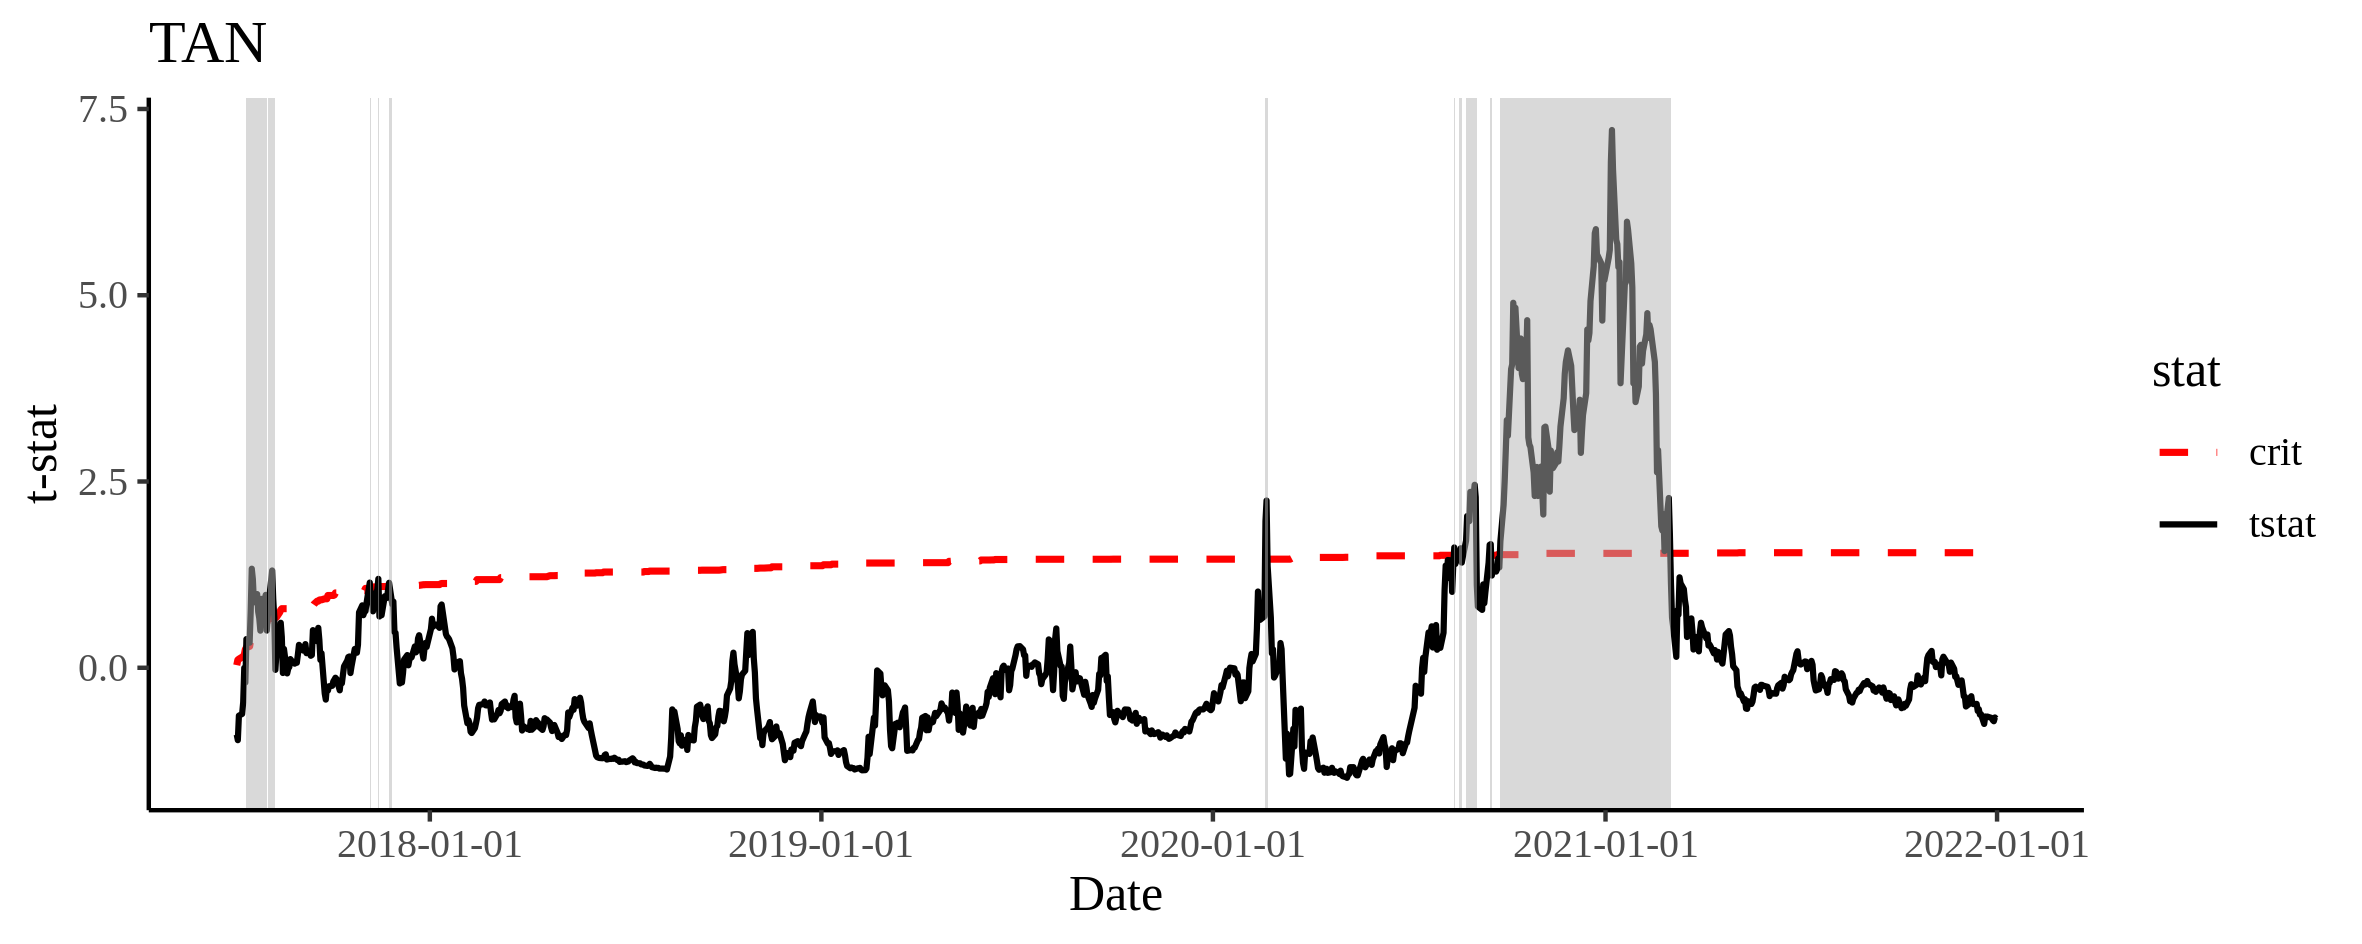
\includegraphics[width=\textwidth]{Figures/gsadf_prediciton.png}
    \caption{GSADF Results}
    \label{fig:GSADF_results}
\end{figure}

Depending on the test, several more regime switches can be observed within the sample period. Both tests have detected explosive price behaviors in Q3 2017, as well as in Q1 2020, just before the crash of the global financial markets. However, the duration of these periods differs depending on the test. All detected bubble episodes can be found in Appendix B (SADF) and Appendix C (GSADF).
\newline

The SADF has detected more smaller bubble episodes as opposed to the GSADF, since the critical values calculated by the Monte Carlo simulations are smaller than those of the GSADF which is to be expected (Monschang \& Wilfling, 2021), whereas the test stastics of both are equal at 7.217. This is why all episodes detected by the SADF were picked up by the GSADF test as well -- most notably the big episode post-March 2020. The former test has placed the origination of the bubble episode sometime after the market crash as markets started to regain momentum, where as the latter has dated the origination later on, following a small sell-off of the initial price momentum. The SADF test also places the burst of the episode later on when the cashing in of the price peak bottomed out in May of 2021, where as the GSADF has marked March 2021 as the end. This makes the SADF-detected episode almost two times longer (200 trading days) than the GSADF one (108 trading days). At first glance both episodes appear too short which will be addressed in the next section. Nevertheless, both tests have managed to indicate price exuberance in the sample period which allows for a deeper discussion on the topic of the presence of a speculative bubble in solar energy stocks.
\newpage

\section{Summary \& Discussion}
This paper has dealt with the topic of investment risk and speculative behavior with regard to companies in the solar energy sector in the five-year period between January 2017 and January 2022. By employing a 5-Factor Fama-French model on the TAN ETF, which mirrors the SUNDIX, a solar energy stock index, this study proves that solar energy stocks carry significant risk. Those willing to take on this risk, however, are rewarded by substantial returns, as evidenced by the TAN's massive gains over this time frame, as opposed to the broader market. This might lead one to believe that more and more investors would be willing to take a bet on the renewable energy sector and more specifically on solar energy, as it is not only a perspective sector, but it is one still heavily backed by the government, which mitigates some of the risk. The study proves with the use of two powerful econometric tests -- the sup-augmented Dickey-Fuller and generalized sup-augmented Dickey-Fuller test, that there have been multiple occurrences of explosive price behavior, which can be indicative of a speculative bubble. Most notably in the period after the March 2020 crash of the global financial world, as markets started to recover the prices of solar stocks have rapidly grown until they have been sold off sometime in 2021. Nonetheless, the levels of the TAN's returns have afterwards remained significantly higher than those of the overall market.
\newline

Some limitations of the paper include the lack of analysis of a broader spectre of risk factors to which solar energy stocks might be exposed, such as other sectors of the economy, prices of raw materials, electricity prices and more. Another drawback of the study is the analysis of nominal stock prices as opposed to prices adjusted for inflation. Inflation has been soaring for the past two years and this is something which should be factored in. Maybe this is a reason why a larger speculative bubble could not be identified within the sample period but rather multiple smaller ones. The analysis can also be conducted on a larger period spanning more years, as is done in other studies, in order to capture a broader picture of how exactly prices of solar stocks have developed.
\newline

The question which still remains unanswered is what drives such investment behavior. One might have to consider three world events from the past 15 years. The first one is the Great recession of 2008, which shook the global economy and its effects are still partially felt over the world. Governments worldwide responded to this recession with central monetary and fiscal policies intended to ease the effects of the crash of the global financial markets and kick-start their economies. More than a decade later some of these measures are still in effect, such as low or negative interest rates intended to drive people away from keeping their money deposited in banks and to encourage more liquidity in the economy. As a result more people have sought after alternative investments, which yield returns higher than the set interest rates and also higher than inflation, with he bond or the stock market being a natural choice for new investors. This can partially be the reason behind the offset of the greatest bull run ever on the US stock markets over the last decade, with almost no industry making an exception. This poses an even more difficult to answer question as to whether there is an even greater asset bubble currently present on the stock market, but this question is out of the scope of this study.
\newline

The next big event relating to the out-performance of solar energy stocks is the signing of the Paris Climate Agreement in 2015. This was the biggest world-wide recognition of the climate-change crisis humanity currently faces. This has brought new-found attention to this issue and has set the precedent for the development of the world economy over the following decades. Moreover, a key component to sticking to the goals of the Paris Climate Agreement lies within renewable energy. With solar making out an ever more significant proportion of the worlds renewable energy generation, a lot of investors might see potential in this technology. The Paris Agreement gives a new layer of legitimacy to solar energy and also further reconfirms strong governmental backing of renewable energy, which might give investors a margin of safety with regard to financial or technological risks, thus making them more risk-tolerant and speculative. 
\newline

The third and final event of significance is the COVID-19 pandemic and its aftermath. Similarly to the Great recession, governments world-wide sought out to provide stimulus packages to its population in order to ease up the closing of the economy and the potential job and/or income loses people faced. For some this government stimulus presented the opportunity to start investing in stocks and other financial derivatives. This coupled with the popularity of zero-commission online or mobile brokers saw the birth of a new generation of retail investors. In an interview for Financial Times (Nauman, 2021) Moses Sutton, a Barclays analyst, suggests that a significant part of the soaring prices in clean energy stems from retail investors since they perceive green energy as "\textit{a well-known brand linked to the energy transition}".
\newline

Clean energy is not and will not be the only sector that is influenced by speculation, however it is a sector of great importance, not only from a financial point of view but also from a social and moral perspective. Financial stability in this sector is crucial if the goal of carbon-neutrality is to be achieved. According to IEA (2021b), in order to reach net-zero emissions by 2050, investments in green energy have to reach \$4 trillion within the next eight years. For this development to be sustainable, sound financial fundamentals need to be established, since the risk of a green-asset bubble inflating and inevitably bursting might not only send shock-waves across financial markets, but might also undo years-worth of development in this sector. This is why policy maker should also shift their focus on establishing frameworks, which hinder speculative trading in the green energy sector, as to not compromise the energy transition world-wide. 

\newpage
\section{References}

Antoniuk, Y., Leirvik, T. (2021) Climate change events and stock market returns. \textit{Journal of Sustainable Finance \& Investment}, p. 1-26
\newline

Bohl, M. T., Kaufmann, P., Siklos, P. L. (2013). From Hero to Zero: Evidence of
Performance Reversal and Speculative Bubbles in German Renewable Energy Stocks.
\textit{Energy Economics} 37, p. 40-51
\newline

Bohl, M. T., Kaufmann, P., Siklos, P. L. (2015). What drove the mid-2000s explosiveness in alternative energy stock prices? Evidence from US, European and global indices.
\textit{International Review of Financial Analysis} 40, p. 194-206
\newline

Bondia R, Ghosh S, Kanjilal K (2016) International crude oil prices and the stock prices of clean energy and technology companies: evidence from non-linear cointegration tests with unknown structural breaks. \textit{Energy} 101, p. 558–565
\newline

Carhart, M. M., (1997) On Persistence in Mutual Fund Performance. \textit{Journal of Finance} 52 (1), p. 57-82
\newline

Dickey, D.A., Fuller, W.A. (1979) Distribution of the Estimators for Autoregressive Time Series with a Unit Root. \textit{Journal of the American Statistical Association} 47, p. 427-431.
\newline

Fama, E. F., French, K. R, (1993) Common risk factors in the returns on stocks and bonds. \textit{ournal of Financial Economics} 33 (1), p. 3-56
\newline

Fama, E. F., French, K. R, (2015) A five-factor asset pricing model. \textit{Journal of Financial Economics} 116 (1), p. 1-22
\newline

FS-UNEP (2020) Global Trends In Renewable Energy Investment 2020. \textit{Frankfurt School of Finance \& Management gGmbH}, Frankfurt am Main
\newline

Henriques, I., Sadorsky, P. (2008) Oil prices and the stock prices of alternative energy companies. \textit{Energy Economics}, 30 (3), p. 998-1010.
\newline

IEA (2020) Renewables 2020, \textit{International Energy Agency}, Paris https://www.iea.org/reports/renewables-2020
\newline

IEA (2021a), World Energy Outlook 2021, \textit{International Energy Agency}, Paris https://www.iea.org/reports/world-energy-outlook-2021

IEA (2021b) Net Zero by 2050, \textit{International Energy Agency}, Paris https://www.iea.org/reports/net-zero-by-2050
\newline

Inchauspe, J., Ripple, R.D., Trück, S. (2015) The dynamics of returns on renewable energy companies: a state-space approach. \textit{Energy Economics}, 48, p. 325-335
\newline

IRENA (2021) Renewable Power Generation Costs In 2020. \textit{International Renewable Energy Agency}, Abu Dhabi
\newline

Kumar, S., Managi, S., Matsuda, A. (2012) Stock Prices of Clean Energy Firms, Oil and
Carbon Markets: A Vector Autoregressive Analysis. \textit{Energy Economics}, 34 (1), p 215-226
\newline

Lintner, J. (1965) The Valuation of Risk Assets and the Selection of Risky Investments in Stock Portfolios and Capital Budgets. \textit{Review of Economics and Statistics} 47, p. 13-37
\newline

Pavlidis, E., Martínez-García, E., Grossman, V. (2019) Detecting periods of exuberance: A look at the role of aggregation with an application to house prices. \textit{Economic Modelling} 80, p. 87-102,
\newline

Phillips, P. C. B., Wu, Y., Yu, J. (2011) Explosive Behavior in the 1990s NASDAQ: When
Did Exuberance Escalate Asset Values? \textit{International Economic Review} 52 (1), p. 201-226
\newline

Phillips, P. C. B., Shi, S., Yu, J. (2015) Testing For Multiple Bubbles: Historical Episodes Of Exuberance And Collapse In The S\&P 500. \textit{International Economic Review} 56 (4), p. 1043 - 1078
\newline

Managi, S. and Okimoto, T., (2013), Does the price of oil interact with clean energy prices in the stock market? \textit{Japan and the World Economy}, 27 (C), p. 1-9
\newline

Monschang, V., Wilfling, B. (2021) Sup-ADF-style bubble-detection methods under test. \textit{Empir Econ} 61, p. 145–172
\newline

Nauman, B. (19.02.2021) ‘Green bubble’ warnings grow as money pours into renewable stocks. \textit{Financial Times}
\newline

Sadorsky, P., 2012a. Correlations and Volatility Spillovers between Oil Prices and the
Stock Prices of Clean Energy and Technology Companies. \textit{Energy Economics} 34 (1), p. 248-255
\newline

Sadorsky, P., 2012b. Modeling Renewable Energy Company Risk. \textit{Energy Policy} 40, p. 39- 48
\newline

Schütze, F., Aleksovski, D., Mozetic, I. (2020) Stock Market Reactions to International Climate Negotiations
\newline

Sharpe, W. (1964) Capital Asset Prices: A Theory Of Market Equilibrium Under Conditions Of Risk. \textit{Journal of Finance} 19 (3), p. 425-442
\newline

Sokolovska, I., Kešeljević, A. (2019) Does sustainability pay off? A multi-factor analysis on regional DJSI and renewable stock indices. \textit{Economic Research-Ekonomska Istraživanja} 32, p. 423-439
\newline

Zhao, X. (2020) Do the stock returns of clean energy corporations respond to oil price shocks and policy uncertainty? \textit{Economic Structures} 9 (53)
\newline


\begin{appendices}

\begin{landscape}
\section{SUNDIX Stocks}
\scriptsize
% Table created by stargazer v.5.2.2 by Marek Hlavac, Harvard University. E-mail: hlavac at fas.harvard.edu
% Date and time: Thu, Mar 31, 2022 - 08:25:10 AM
\begin{longtable}{ *{9}{l} }
  \caption{List of stocks and their respective weights listed in the SUNDIX. Data from https://macsolarindex.com/stocks-in-the-index/} 
  \label{SUNDIX_stocks} 
\\[-1.8ex]
\hline \\[-1.8ex] 
 & As of 29 Mar 2022 & Bloomberg Ticker & Stock Exchange & Headquarters & Stock Currency & Exposure Factor & Solar revenue above 50\% & Weight \\ 
\hline \\[-1.8ex] 
1 & Enphase Energy Inc & ENPH:US & Nasdaq & US & USD & $1$ & yes & 11.44\% \\ 
2 & SolarEdge Technologies Inc & SEDG:US & Nasdaq & US & USD & $1$ & yes & 9.76\% \\ 
3 & First Solar Inc & FSLR:US & Nasdaq & US & USD & $1$ & yes & 6.57\% \\ 
4 & Sunrun Inc. & RUN:US & Nasdaq & US & USD & $1$ & yes & 5.73\% \\ 
5 & Xinyi Solar Holdings Ltd & 968:HK & Hong Kong & China & HKD & $1$ & yes & 5.73\% \\ 
6 & GCL-Poly Energy Holdings Ltd & 3800:HK & Hong Kong & China & HKD & $1$ & yes & 5.60\% \\ 
7 & Daqo New Energy Corp & DQ:US & NYSE & China & USD & $1$ & yes & 3.79\% \\ 
8 & JinkoSolar Holding Co Ltd & JKS:US & NYSE & China & USD & $1$ & yes & 3.24\% \\ 
9 & Sunnova Energy International Inc & NOVA:US & NYSE & US & USD & $1$ & yes & 2.79\% \\ 
10 & Atlantica Sustainable Infrastructure plc & AY:US & Nasdaq & UK & USD & $1$ & yes & 2.68\% \\ 
11 & Hannon Armstrong Sustainable Infrastructure & HASI:US & NYSE & US & USD & $0.500$ & no & 2.61\% \\ 
12 & Encavis AG & ECV:GR & Xetra & Germany & EUR & $1$ & yes & 2.51\% \\ 
13 & Shoals Technologies Group - Class A & SHLS:US & Nasdaq & US & USD & $1$ & yes & 2.50\% \\ 
14 & Hanwha Solutions & 009830:KS & Korea SE & South Korea & KRW & $0.500$ & no & 2.35\% \\ 
15 & Array Technologies Inc. & ARRY:US & Nasdaq & US & USD & $1$ & yes & 2.34\% \\ 
16 & Canadian Solar Inc & CSIQ:US & Nasdaq & China & USD & $1$ & yes & 2.32\% \\ 
17 & Sunpower Corp & SPWR:US & Nasdaq & US & USD & $1$ & yes & 2.27\% \\ 
18 & Xinyi Energy Holdings Ltd & 3868:HK & Hong Kong & China & HKD & $1$ & yes & 1.93\% \\ 
19 & Flat Glass Group Co Ltd - H Shares & 6865:HK & Hong Kong & China & HKD & $1$ & yes & 1.88\% \\ 
20 & Solaria Energia y Medioambiente SA & SLR:SM & Madrid & Spain & EUR & $1$ & yes & 1.81\% \\ 
21 & Enlight Renewable Energy Ltd & ENLT:IT & Tel Aviv & Israel & ILS & $0.500$ & no & 1.64\% \\ 
22 & United Renewable Energy Co Ltd & 3576:TT & Taiwan & Taiwan & TWD & $1$ & yes & 1.63\% \\ 
23 & Neoen SA & NEOEN:FP & Euronext Paris & France & EUR & $0.500$ & no & 1.48\% \\ 
24 & Scatec ASA & SCATC:NO & Oslo & Norway & NOK & $0.500$ & yes & 1.37\% \\ 
25 & Meyer Burger Technology AG & MBTN:SW & SIX Swiss Ex & Switzerland & USD & $1$ & yes & 1.26\% \\ 
26 & SMA Solar Technology AG & S92:GR & Xetra & Germany & EUR & $1$ & yes & 1.13\% \\ 
27 & TSEC Corporation & 6443:TT & Taiwan & Taiwan & TWD & $1$ & yes & 1.07\% \\ 
28 & West Holdings Corp & 1407:JP & Tokyo & Japan & JPY & $0.500$ & no & 0.94\% \\ 
29 & O.Y. Nofar Energy Ltd & ENRG:IT & Tel Aviv & Israel & ILS & $1$ & yes & 0.88\% \\ 
30 & Energix - Renewable Energies Ltd & ENRG:IT & Tel Aviv & Israel & ILS & $0.500$ & no & 0.87\% \\ 
31 & Azure Power Global & AZRE:US & NYSE & India & USD & $1$ & yes & 0.82\% \\ 
32 & Motech Industries Inc & 6244:TT & Taipei & Taiwan & TWD & $1$ & yes & 0.81\% \\ 
33 & RENOVA Inc & 9519:JP & Tokyo & Japan & JPY & $0.500$ & yes & 0.80\% \\ 
34 & Luoyang Glass H HKD & 1108:HK & Hong Kong & China & HKD & $1$ & yes & 0.78\% \\ 
35 & Maxeon Solar Technologies Ltd & MAXN:US & Nasdaq & Singapore & USD & $1$ & yes & 0.76\% \\ 
36 & ReneSola Ltd ADR & SOL:US & NYSE & US & USD & $1$ & yes & 0.67\% \\ 
37 & Doral Group Renewable Energy Resources & DORL:IT & Tel Aviv & Israel & ILS & $1$ & yes & 0.64\% \\ 
38 & Giga Solar Materials Corp & 3691:TT & Taipei & Taiwan & TWD & $1$ & yes & 0.59\% \\ 
39 & Grenergy Renovables & GRE:SM & Madrid & Spain & EUR & $0.500$ & yes & 0.55\% \\ 
40 & Beijing Enterprises Clean Energy Group Limited & 1250:HK & Hong Kong & China & HKD & $0.500$ & yes & 0.51\% \\ 
41 & GCL New Energy Holdings Ltd & 451:HK & Hong Kong & Hong Kong & HKD & $1$ & yes & 0.49\% \\ 
42 & SOLTEC POWER HOLDINGS S.A & SOL:SM & Madrid & Spain & EUR & $1$ & yes & 0.46\% \\ 
\hline \\[-1.8ex] 
\end{longtable} 

\end{landscape}
\newpage

\section{SADF Bubble Episodes}
% Date and time: Fri, Apr 01, 2022 - 09:11:12 AM
\begin{table}[!htbp] \centering 
  \caption{} 
  \label{} 
\begin{tabular}{@{\extracolsep{5pt}} cccc} 
\\[-1.8ex]\hline 
\hline \\[-1.8ex] 
 & Start & End & Duration \\ 
\hline \\[-1.8ex] 
1 & 2017-07-14 & 2017-08-10 & $19$ \\ 
2 & 2017-08-11 & 2017-08-17 & $4$ \\ 
3 & 2017-08-18 & 2017-08-21 & $1$ \\ 
4 & 2017-08-31 & 2017-09-12 & $7$ \\ 
5 & 2017-09-14 & 2017-09-21 & $5$ \\ 
6 & 2017-09-22 & 2017-09-25 & $1$ \\ 
7 & 2017-10-23 & 2017-12-04 & $29$ \\ 
8 & 2017-12-11 & 2017-12-12 & $1$ \\ 
9 & 2017-12-14 & 2018-01-24 & $26$ \\ 
10 & 2020-02-11 & 2020-02-27 & $11$ \\ 
11 & 2020-03-04 & 2020-03-06 & $2$ \\ 
12 & 2020-07-15 & 2020-07-16 & $1$ \\ 
13 & 2020-07-17 & 2021-05-04 & $200$ \\ 
14 & 2021-06-24 & 2021-07-14 & $13$ \\ 
15 & 2021-08-03 & 2021-08-05 & $2$ \\ 
16 & 2021-08-09 & 2021-08-10 & $1$ \\ 
17 & 2021-10-27 & 2021-11-10 & $10$ \\ 
18 & 2021-11-11 & 2021-11-23 & $8$ \\ 
\hline \\[-1.8ex] 
\end{tabular} 
\end{table}  
\newpage

\section{GSADF Bubble Episodes}
% Table created by stargazer v.5.2.2 by Marek Hlavac, Harvard University. E-mail: hlavac at fas.harvard.edu
% Date and time: Fri, Apr 01, 2022 - 09:09:59 AM
\begin{table}[!htbp] \centering 
  \caption{} 
  \label{} 
\begin{tabular}{@{\extracolsep{5pt}} cccc} 
\\[-1.8ex]\hline 
\hline \\[-1.8ex] 
 & Start & End & Duration \\ 
\hline \\[-1.8ex] 
1 & 2017-07-14 & 2017-08-02 & $13$ \\ 
2 & 2017-08-03 & 2017-08-10 & $5$ \\ 
3 & 2017-11-06 & 2017-11-07 & $1$ \\ 
4 & 2017-11-14 & 2017-11-15 & $1$ \\ 
5 & 2017-11-24 & 2017-11-27 & $1$ \\ 
6 & 2020-02-19 & 2020-02-21 & $2$ \\ 
7 & 2020-08-13 & 2020-08-14 & $1$ \\ 
8 & 2020-08-17 & 2020-08-20 & $3$ \\ 
9 & 2020-08-24 & 2020-09-03 & $8$ \\ 
10 & 2020-09-15 & 2020-09-17 & $2$ \\ 
11 & 2020-09-25 & 2021-03-03 & $108$ \\ 
\hline \\[-1.8ex] 
\end{tabular} 
\end{table} 

\end{appendices}

\end{document}